\documentclass[a4paper,12pt]{article}
\usepackage{uppsats}

\addbibresource{referenser.bib}
\figurer[.jpg,.pdf]{./figurer/}

\uppsatstitel{Fältbussar}
\forfattare{Alexander Nilsson}
\kurs{Datorteknik 1a}
\skola{Hermods}
\logotyp{logo}

\makeatletter
\def\@maketitle{
  \raggedright
  \includegraphics[\@logotypalt]{\@logotyp}\par\medskip
  \begin{center}
    {\Huge \bfseries \@uppsatstitel }\par
    {\Large \bfseries \@forfattare}\par
    {\large \@kurs}\par
    {\large \@skola}\par\medskip
    {
      \IfValueTF{\@revdatum}{
        % pubdatum med revdatum
        \@pubdatum (rev. \@revdatum)
      }{
        \@pubdatum
      }
    }\par\bigskip
  \end{center}
}
\makeatother

\pagestyle{fancy}
\fancyhead{}
\fancyhead[L]{}
\fancyhead[R]{\bfseries \footnotesize \MakeUppercase{\articlename}}
\renewcommand{\headrulewidth}{0pt}
\fancyfoot{}
\fancyfoot[L]{}
\fancyfoot[R]{\bfseries \small \thepage}

\begin{document}

\maketitle
\pagenumbering{gobble}
\thispagestyle{empty}
\clearpage

\pagenumbering{arabic}

\begin{multicols}{2}

\section{Inledning}

Fältbussar är en teknologi för anslutning av enheter i ett centralt eller distribuerat kontrollsystem. Enheter kan vara fältenheter så som sensorer och ställdon, och fältkontroller så som programmerbara styrsystem och regulatorer.

Teknologin används i olika industrier för att åstadkomma fabriksautomatisering och processkontrollering och automatisering av system i offentliga lokaler samt i hemmet (\enquote{smarta hem}) \cite[s. 22-25]{distributedfieldbuscontrolnetworksystems}.

Beroende på användningsområdet finns det olika krav på fältbussen, till exempel i området för fabriksautomatisering krävs det låga överföringstider som uppnås genom att använda ett färre antal fältenheter, korta ner längden på bussen och minska på storleken av datapaketen, medan automatisering av lokaler har större krav på pålitlighet och kostnadsbesparingar.

I denna essän kommer jag utforska standarderna för fältbussar, hur de relaterar till OSI-modellen och lite om skillnaderna mellan standarderna samt hur Raspberry Pi (\enquote{Hallonpajen}) kan tänkas tillämpas i ett kontrollsystem eller för dylik automatisering.

\section{Fördjupning}

Fältbussar används bland annat inom områden för industriell mätning, exempelvis i kraftverk för att sända mätningar och diverse signaler till och från flera enheter samtidigt.

Den tekniska lösningen för kommunikation med gränssnittet kan se olika ut beroende på vilken standard man väljer att adaptera sig efter.

\subsection{Open Systems Interconnection}

\subsubsection{Standardisering}

Internationella organisationen för standarder (ISO) publicerar standarden \textit{ISO/IEC 7498} --- eller \textit{Open Systems Interconnection (OSI)} --- som fastställer en specifikation för hur ett öppet system ska anslutas \cite{iso74981}.

Modellen bestämmer hur komponenter i ett öppet system ansluter till varandra, men komponenternas interna funktionalitet och konstruktion faller utanför modellens omfång. 

% \begin{Figure}
% 	\centering
% 	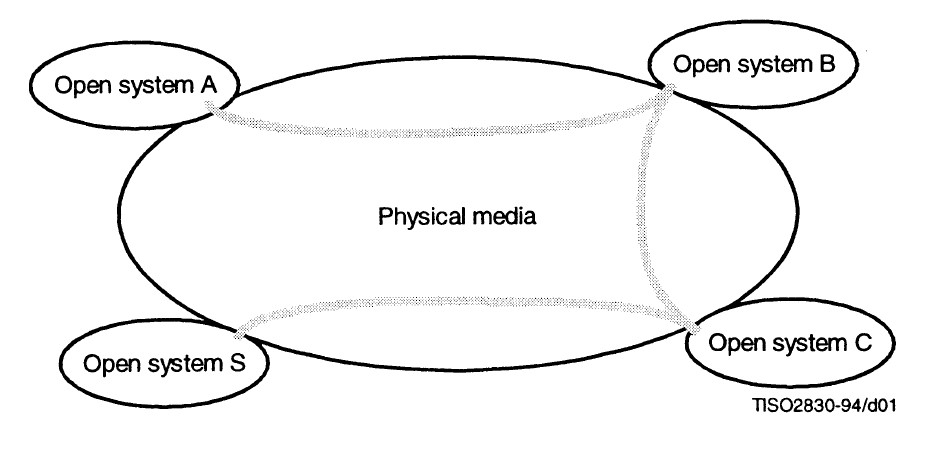
\includegraphics[width=\linewidth]{osianslutningar}
% 	\captionof{figure}{Förbindning av system i OSI-modellens\ccitetitle[s. 3]{iso74981}}
% \end{Figure}

OSI-modellen specificerar sju lager i arkitekturen för kommunikation:

\begin{enumerate}[label={\bfseries(\arabic*)}]
	\item Fysiska lagret: ansvarar för att sända och motta rå data mellan enheten och det fysiska mediumet
	\item Datalänk-lagret: ansvarar för kommunikation mellan noder och korrigering av fel som kan uppstå i fysiska lagret
	\item Nätverkslagret: ansvarar för överföring av datasekvenser --- paket --- mellan noder i nätverk
	\item Transportlagret: ansvarar för transport av datasekvenser från källa till destination utan kvalitetsförlust
	\item Sessionslagret: ansvarar för att hålla reda på dialoger mellan värder
	\item Presentationslagret: ansvarar för att hålla reda på kontext mellan applikationlager-entiteter 
	\item Applikationslagret: ansvarar för kommunikation med programvaran, lagret närmast användaren
\end{enumerate}

\subsubsection{Fältbussar}

% Kablage samt lager 1, 2 och 7

Fältbussens standard avgörs utifrån fysiska mediumet av kablage, samt fysiska lagret, datalänk lagret och applikationslagret enligt OSI-referensmodellen. 

% \begin{Figure}{faltbusfysisktlager}[faltbusfysisktlager]
% 	Relation till fysiska lagret av fältbussens nätverksarkitektur
% 	\ccitetitle[s. 884]{mapepa}
% \end{Figure}

\textit{\MakeUppercase{Foundation} Fieldbus H1}-standarden  skiljer sig till exempel märkbart mot \textit{PROFIBUS DP}-standarden (eng. \textit{decentralised peripherals}) vad gäller prestanda, men \textit{PROFIBUS PA}-standarden \footnote{PROFIBUS PA tillämpar standarden IEC 61158-2 \cite{profibuspowerplants} \cite[s. 1083]{fieldbustechindustrialautomation}.} (eng. \textit{process automation}) har ungefär jämlik prestanda. Poängen jag försöker nå är att området \enquote{fältbussar} är ett väldigt komplext ett och det är inte lätt att kortfattat beskriva exakt hur en fältbuss används i nätverk för att det skiljer sig starkt från standard till standard.

\subsection{Hallonpajen}

Hallonpajen kan i ett öppet kontrollsystem anslutas som en fristående fältkontroller med ett \enquote{integrerat} programmatisk styrsystem och kommunikationsmöjligheter \footnote{Raspberry Pi 4 model B har kommunikationsprotokollen IEEE 802.11ac WLAN, Gigabit ethernet, Bluetooth 5.0 och BLE, 2xUSB2.0, 2xUSB3.0.} med bandbredder som väl möter dagens krav. Folk inom industrin (tillverkning, m.fl.) talar gott om Hallonpajen, men med viss tveksamhet angående riskerna att bryta från industristandarderna och förlora den kritiska support från leverantörer som man förlitar sig på \cite{raspberrypireadyforindustry}.

En annan kritisk begränsning i att sätta in en Hallonpaj i en verklig industriprocess är kompatabilitet mellan olika kommunikationsstandarder som kanske inte stöds \enquote{out-of-the-box} av Hallonpajen (se figur \ref{fig:raspberrypiprofibusdp}).

\begin{minipage}{\linewidth}
		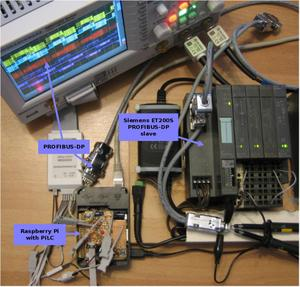
\includegraphics[width=\linewidth]{pilc_et200s}
		\captionof{figure}{Hallonpaj som interfacar med PROFIBUS DP \cciteauthorfull{raspberrypiprofibus}}
		\label{fig:raspberrypiprofibusdp}
\end{minipage}

\subsubsection{Hallonpajen som styrenhet i hemmet}

Även om Hallonpajen inte ännu är helt redo för industriellt bruk så används den flitigt inom hemautomatisering (\enquote{smarta hem}), till exempel för att styra belysning, klimatanläggningar och säkerhetssystem via mobilapplikationer eller med automatisering (övervaka inomhusklimat och justera AC:n, ställa in ljustemperatur efter tid på dygnet, etc.) \cite{iotsmarthomeautomation}.

\end{multicols}

\clearpage\printbibliography

\end{document}
